\section{Набор данных (Dataset)}
\label{sec:dataset}

В данной работе представлен датасет $D_u$, состоящий из фундаментально двух разных доменов. Первая его часть 
покрывает параграфы $d_i$ из таких вселенных, как ``Гарри Поттер'', ``Голодные игры'', ``Преступление и наказание'', диалоги из фрагментов игр - ``Ведьмак: Дикая охота'', ``Need For Speed: Most wanted (2005)'' и многие другие.
Вторая часть примеров-параграфов $D_v$ - это общеизвестные параграфы из истории, науки или же просто факты.
Такая вариативность позволяет более объективно оценить предложенный алгоритм и сравнить его на каждом из наборе данных отдельно и в совокупности - $D_{uv}$. 


\subsection{Обзор данных}

Наборы данных $D_u$ и $D_v$ представлены в разном семантическом стиле описания, грамматики, и изложения. Так, например, $D_u$ - 
представляет собой набор данных, преимущественно из фэнтезийных произведений и классики русской литературы. Стиль изложения и использование 
специфичных имен собственных - названия стран, городов, прямая речь героев и их диалоги, отличающихся сильным контрастом от 
более формального стиля изложения.  В таблице \eqref{tab:countdist} представлно распределение вопросов и параграфов по каждой из вселенной.

\begin{table}[h]
    \centering
    \begin{tabular}{l|ccccc}
        \textbf{} & \textbf{$|Q|$} & \textbf{$|D|$}  \\
        \hline
        \textbf{$D_{u}$}  &$14498$ &$4992$  \\
        \textbf{$D_{v}$}  &$9910$  &$4425$ \\
    \end{tabular}
    \caption{Распределение запросов $Q$ и параграфов $D$ по количеству относительно $D_u$ и $D_v$}
    \label{tab:countdist}
\end{table}

Таким образом, весь набор данных состоит из \textbf{$4992 + 4425=9417$} уникальных параграфов, из  которых $2496$ представлены на англиском языке, и 
\textbf{$24408$} корректно составленных к ним вопросов, среди которых $7249$ составлены на английском языке. Добавление разных языков повествования дополнительно добавляет 
морфологическую сложность, т.к. многие параграфы имеют очень схожее повествование и контекст, однако написаны на разных языках. Корректным будет считаться, разумеется, только тот параграф, который написан на том же языке, что и заданный к нему вопрос.

Для демонстрации стилистического сдвига  представлена кластеризация подмножества $\hat{D} \subseteq D_u + D_v$. Для векторного отображения была выбрана 
базовая модель $E5_{base}$ \cite{e5}, которая сопоставляет каждому параграфу $d_j \in \hat{D}$ - вектор $\vec{v}_j \in \Re^{768}$, который сначала 
проецируется на под-пространство $\Re^{768} \mapsto \Re^{10}$, используя алгоритм \textit{UMAP} \cite{UMAP}. Полученные проецированные вектора, затем, 
кластеризуются через \textit{HDBSCAN} \cite{HDBSCAN} и визуализация представлена ниже.

% Обычная вставка изображения в одну колонку
\begin{figure}[ht]
    \centering
    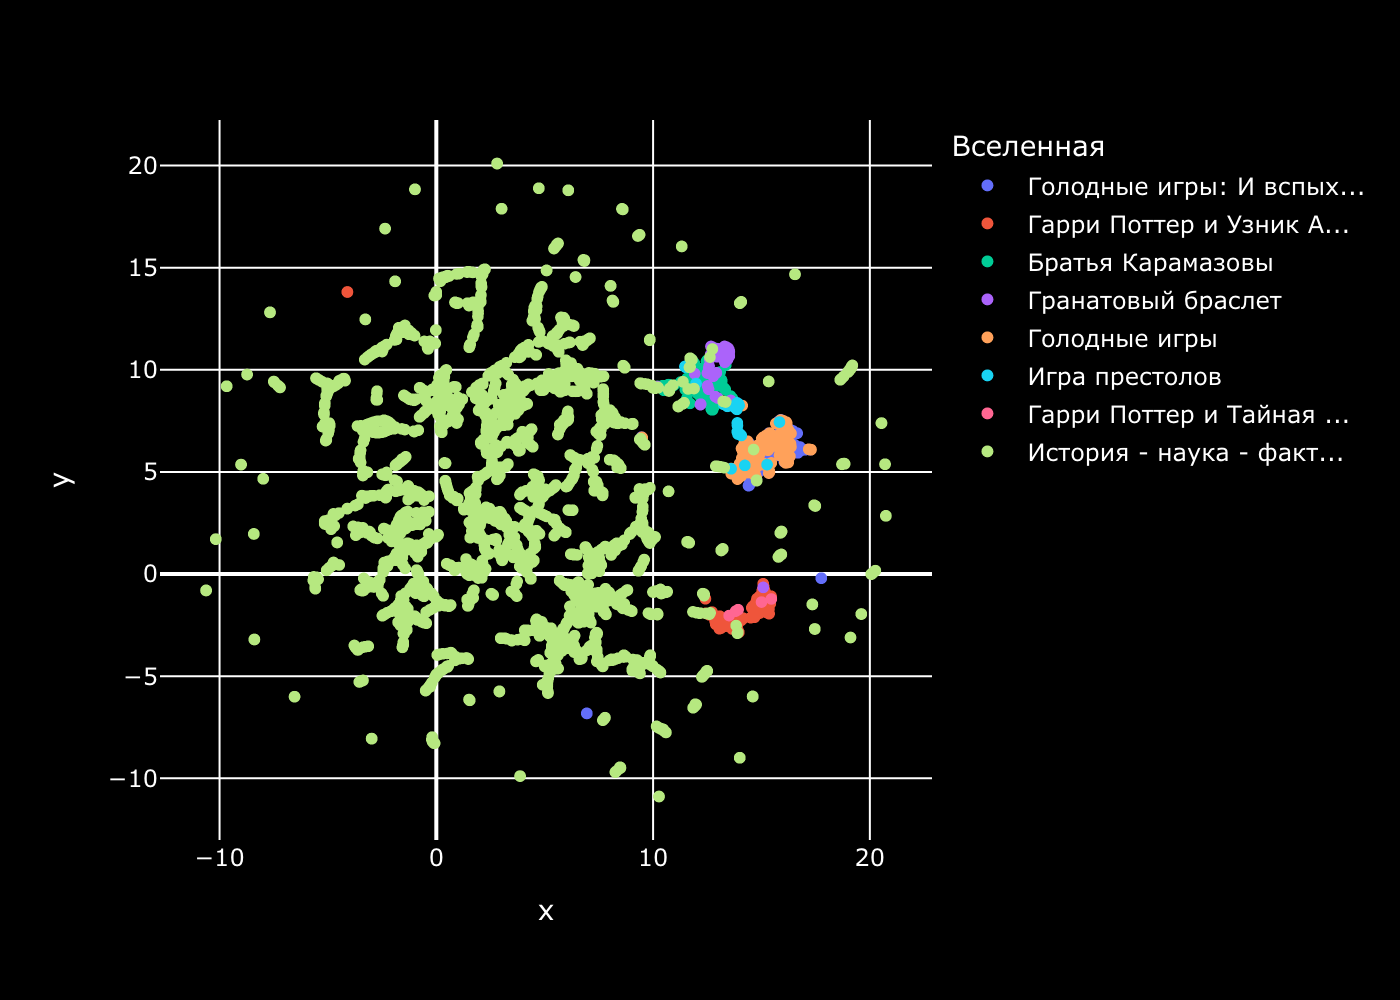
\includegraphics[width=\columnwidth]{figures/clustering-e5-base.png} % Используем ширину одной колонки
    \caption{Кластеризация полного набор данных $D$, включающего в себя как $D_u$,  так и $D_v$}
    \label{fig:clustering-e5-base}
\end{figure}

Ниже представлена таблица \eqref{tab:tokensdist} со статистикой по распределению длин параграфов, запросов, ключевых слов и их пересечения.

\paragraph{Обозначения}
Для каждого параграфа $d_j$ имеется соответствие: $I_j$ - список индексов вопросов $q_i$, ответ на которые содержится в $d_j$. 
Кроме того, каждому параграфу $d_j$ сопоставлены ключевые слова и объяснения $K_j$.

Формально, для каждого параграфа $d_j$ имеется (возможно пустое) множество ключевых слов и их контекстных объяснений, которые обозначются как 
$k_s$ и $e_s$.

\begin{align}
K_j = \{(k^j_{s1}, e^j_{s1}), (k^j_{s2}, e^j_{s2}), \cdots\}
\end{align}

Отметим,что каждое ключевое слово $k_s$ является строгой подстрокой параграфа $k_s \subset d_j$, а объяснение $e_s$, в общем случае, не обязано - $e_s \not\subset d_j$
\paragraph{Статистика}
% \begin{align}
%     L_{Q} &= \frac{1}{|Q|}\sum_{i=1}^{|Q|} |q_i| \\
%     L_{D} &=\frac{1}{|D|}\sum_{j=1}^{|D|} |d_j| \\
%     L_{QD} &= \sum_{j=1} \sum_{i\in I_j} \frac{|q_i \cap d_j|}{|d_j|} \\
%     L_{KD} &= \sum_{j=1} \sum_{s\in K_j} \frac{|k_s \cap d_j|}{|d_j|} \\
%     L_{KED} &= \sum_{j=1} \sum_{s\in K_j} \frac{|k_s \cup e_s \cap d_j|}{|d_j|}
%     \label{eq:coverage}
% \end{align}
\begin{equation}\label{eq:coverage}
    \begin{aligned}
        L_{Q} &= \frac{1}{|Q|}\sum_{i=1}^{|Q|} |q_i|, \\
        L_{D} &= \frac{1}{|D|}\sum_{j=1}^{|D|} |d_j|, \\
        L_{QD} &= \sum_{j=1} \sum_{i \in I_j} \frac{|q_i \cap d_j|}{|d_j|}, \\
        L_{KD} &= \sum_{j=1} \sum_{s \in K_j} \frac{|k_s \cap d_j|}{|d_j|}, \\
        L_{KED} &= \sum_{j=1} \sum_{s \in K_j} \frac{|k_s \cup e_s \cap d_j|}{|d_j|}.
    \end{aligned}
\end{equation}
В уравнениях \eqref{eq:coverage} определяются статистики, важные для подсчета и обоснования важности учета алгоритма (мотивы их ввода более подробно объяснены далее). 
$L_{Q}, L_{D}$ - это длины (среднее) запросов и параграфов соответственно. $L_{QD}$ - среднее покрытие (пересечение) слов из запросов с релевантными параграфами.
$L_{KD}, L_{KED}$ - это процент покрытия токенов параграфа его соответствующими ключевым словами (без объяснениний) и ключевыми словами вместе с объяснениями.
\begin{table}[h]
    \centering
    \begin{tabular}{l|ccccc}
        \textbf{} & \textbf{$L_{Q}$} & \textbf{$L_{D}$} & \textbf{$L_{QD}$} & \textbf{$L_{KD}$} & \textbf{$L_{KED}$} \\
        \hline
        \textbf{$D_{u}$}  &$22.48$ &$144.125$  &$4.77\%$  &$8.64\%$  & $21.45\%$ \\
        \textbf{$D_{v}$}  &$24.99$  &$100.73$  &$6.03\%$  &$8.96\%$  & $23.69\%$ \\
        \textbf{$D_{uv}$} &$23.66$  &$123.73$  &$5.3\%$  &$8.79\%$  & $22.5\%$ \\
    \end{tabular}
    \caption{Распределение ключевых статистических метрик относительно $D_u$ и $D_v$ наборов данных}
    \label{tab:tokensdist}
\end{table}

Несмотря, на очевидную разницу двух наборов данных -  $L_D(D_u)=144.125$ и $L_D(D_v)=100.73$, их стилистику, речевые обороты и другие лингвистические характеристики, отдельно взятый набор $D_u$ сам по себе уникален с точки зрения поиска. 
Так, например, ниже представлена кластеризация подмножества $\hat{D_u} \subset D_u$ произведений $D_u$ в количестве $|\hat{D_u}|=1530$ примеров.

\begin{figure}[ht]
    \centering
    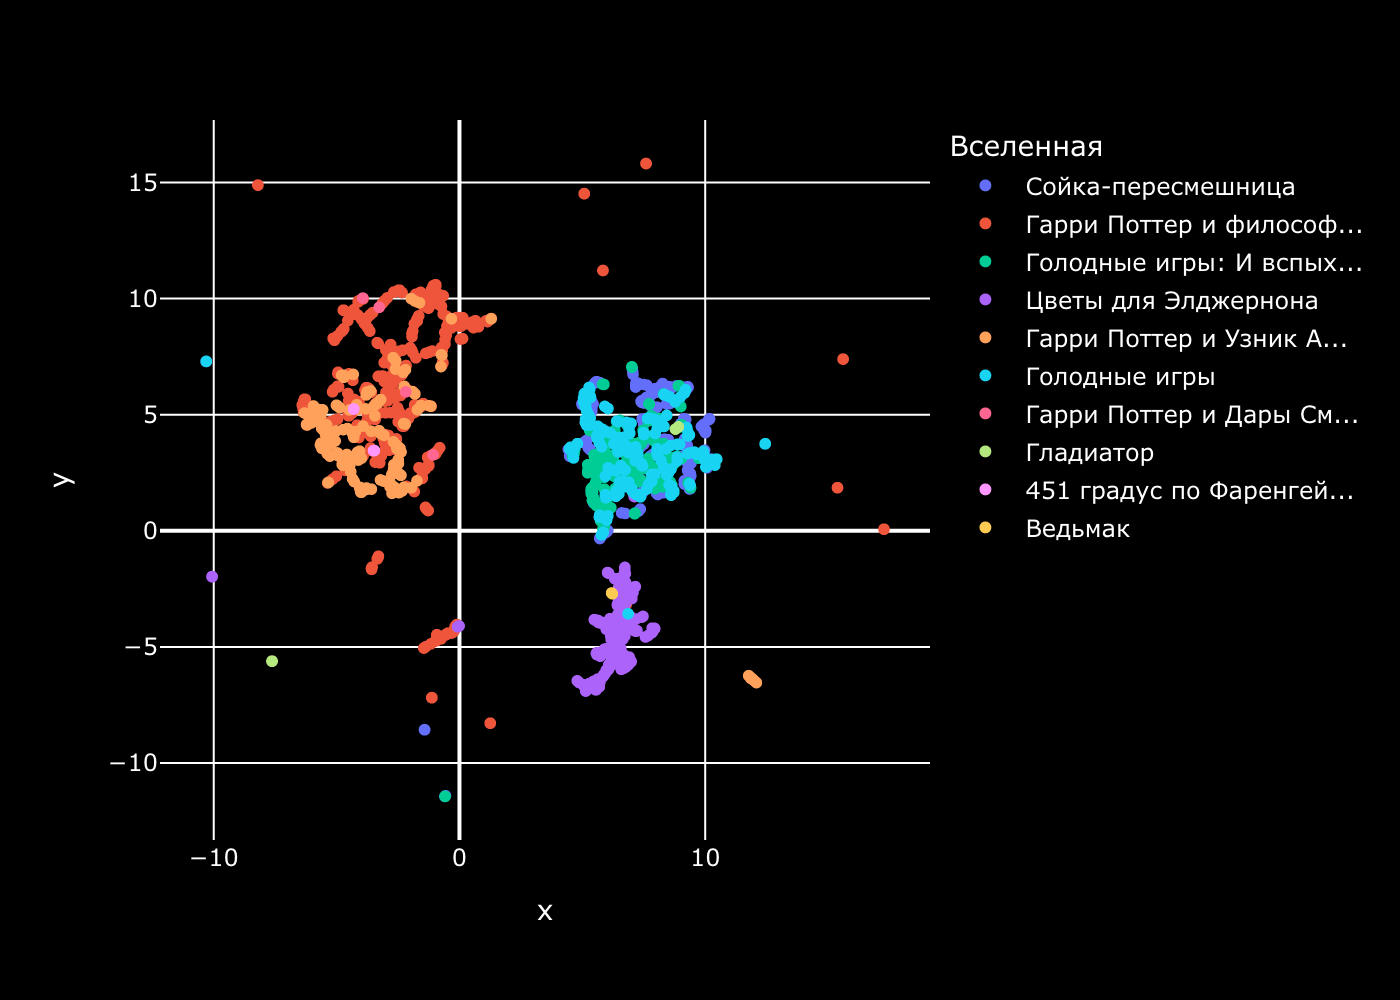
\includegraphics[width=\columnwidth]{figures/clustering_model=[e5]_dataset=[universe].png} % Используем ширину одной колонки
    \caption{Демонстрация кластеризации набора данных $D_u$}
    \label{fig:clustering-e5-base-universe}
\end{figure}